% !TEX root = DataDrivenBayes.tex
 

\section*{Introduction}

Over the last two decades, Bayesian models have emerged as a powerful tool for understanding human cognition. Taking inspiration from Marr's \citeyear{marr_vision_1982} notion of computational level models and Anderson's \citeyear{anderson_adaptive_1990} outline of a rational analysis, the key idea is to take a top-down view of model construction. Within this program, human cognition is viewed in terms of the solution to a computational problem posed by the environment in which humans operate. This approach to cognitive modeling has been successfully applied to a wide range of problems in concept learning \cite{tenenbaum_bayesian_1999}, reasoning \cite{oaksford_rational_1994}, causal inference \cite{griffiths_structure_2005}, perception \cite{knill_perception_1996,shen2016}, motor control \cite{kording_bayesian_2004}, social cognition \cite{baker_action_2009}, decision making \cite{vul_one_2014}, language acquisition \cite{perfors_learnability_2011}, and many more besides. In general, computational-level analyses can take many forms. The existing literature includes analyses that rely on information theory \cite<e.g.,>{navarro_hypothesis_2011}, reinforcement learning \cite<e.g.,>{NavarroSUB}, algorithmic complexity theory \cite<e.g.,>{chater_generalized_2003_FIXED}, and statistical decision theory \cite<e.g.,>{vul_one_2014}, among others. However, the majority of computational-level analyses are framed in {\it Bayesian} terms. 

Bayesian analyses typically approach human learning and reasoning by assuming that the learner's task is to infer which hypothesis $h$ among many possibilities best characterizes the world. The collection of possible hypotheses $\bigh$ is referred to as the {\it hypothesis space}, and the learner's pre-existing beliefs are captured by a {\it prior distribution} $P(h)$. Upon encountering data $x$, the learner updates her beliefs to a {\it posterior distribution} $P(h|x)$ via Bayes' rule:
\be
P(h|x) = \frac{ P(x|h) P(h) }{\sum_{h^\prime \in \bigh} P(x|h^\prime) P(h^\prime)}
\label{eq:bayes}
\ee
This belief updating rule relies heavily on the {\it likelihood function} $P(x|h)$, which describes the probability that the learner would have observed data $x$ if hypothesis $h$ were true. The likelihood function is what allows the learner to make inductive leaps, transforming her prior beliefs $P(h)$ into posterior beliefs $P(h|x)$ that have been informed by data. One of the distinctive characteristics of the Bayesian framework for cognitive modeling is the fact that belief revision via Bayes' rule is often described as a uniquely coherent way to reason rationally from data \cite<e.g.,>{jaynes_probability_2003}, a virtue that is reflected in the growing psychological literature on Bayesian data analysis \cite<e.g.,>{lee_bayesian_2014,kruschke_doing_2010,rouder_default_2012}. 

Highlighting the success of the framework, there are now a number of tutorial articles \cite{perfors_tutorial_2011} and overviews \cite{tenenbaum_theory-based_2006}, as well as a number of papers articulating concerns and disagreements with the Bayesian approach \cite{jones_bayesian_2011,bowers_bayesian_2012,marcus_how_2013, CasseySUB}, defences of the paradigm \cite{chater_imaginary_2011,griffiths_how_2012,goodman_relevant_2015}, and responses to those defences \cite{bowers_is_2012,marcus_still_2015,jones_pinning_2011}. The scope of this debate is broad, but two concerns in particular stand out in these discussions. First, critics of the Bayesian approach frequently take issue with substantive claims about the optimality of human cognition. Second, a common criticism is that Bayesian models are too unconstrained, and that virtually any pattern of behavior can be accommodated by a suitably-formulated Bayesian model. The two criticisms combine to produce the worry that Bayesian models of cognition make a central claim about optimality that is unfalsifiable: that it is always possible to ``prove'' that humans are rational by judicious choice of priors and likelihoods. If this were true, the result would be a modeling framework that is not only vacuous, but also does not make an interesting claim about human psychology.

This critique exposes a degree of tension in how Bayesian models are constructed and the scientific inferences they license about human cognition. Our claim is that there are two quite different ways of thinking about Bayesian cognitive models: A model might act as a normative standard against which human cognition is measured, or it might serve as as a descriptive tool used to instantiate theories about human cognition \cite<see, e.g.,>{mckenzie_rational_2003}. In this paper we argue that the differences between these two perspectives can lead researchers to construct models with very different characteristics. With this in mind, we suggest that it would be useful to make a clear distinction between {\it optimal} Bayesian cognitive models that specify normative standards and license claims about the rationality of human cognition, and {\it descriptive} Bayesian cognitive models that may serve other theoretical goals but do not necessarily have much to say about whether human cognition is rational. 

One reason for introducing the distinction between optimal and descriptive models  is that it is not always obvious when a Bayesian model is intended to imply a normative claim and when it is not: The same terminology is used to describe Bayesian models no matter what implications those models might have for the optimality of human cognition. A second reason for doing so is that it motivates an examination of what role a Bayesian model can play when it is used as a purely descriptive tool, rather than serving as a vehicle for arguments over whether people are ``rational''. By deliberately setting aside any claims to optimality, a descriptive Bayesian approach shifts the research focus away from questions about rationality or optimality, and onto more traditional psychological questions. What biases and beliefs do people bring to a task? (questions about priors) How do people update their knowledge in light of new data? (questions about likelihoods) What representations do people have? (questions about hypothesis spaces) Within the descriptive framework it is possible to learn about these questions by performing inference on those aspects of the model directly, rather than indirectly and in a more {\it ad hoc} way by setting them and examining model fit. The descriptive approach offers a vision for Bayesian cognitive modeling that disentangles the formal apparatus of Bayesian models (with their use of priors, likelihoods, and hypothesis spaces, all of which we want to keep) with the claims about rationality which---while an important foundation of the optimal Bayesian approach---are not required in the descriptive approach.

Our goal in this paper is not to argue for the superiority of either kind of Bayesian model---normative standards and descriptive models are both useful tools for cognitive scientists---but to try to highlight the importance of maintaining a clear distinction. This distinction is theoretical more so than methodological: Although the descriptive approach is much more flexible---and therefore allows for a wider range of methodological approaches to parameter estimation and model selection---this flexibility is \textit{the result} of letting go of optimal interpretations and the constraints that come with them.

With this in mind, we present three illustrative case studies, each chosen to highlight different ways in which the descriptive approach can enable modelers to ask {\it different} questions than a Bayesian model that focuses on questions of optimality.  Our examples show that a descriptive approach allows the researcher to use empirical data to robustly learn the mental representations that underpin human performance. We demonstrate how it can be used to investigate the biases and mental representations that shape human judgments as well as the learning rules that people use to change those beliefs. We examine how individual differences in cognition can be explored within the data-driven, descriptive Bayesian approach. Finally, our examples show that the insights obtained with a descriptive approach can be compared and contrasted with the findings of an optimal model---sometimes lending support and sometimes standing in opposition---or that they can stand alone without consideration to questions of optimality.


\subsection*{What makes a Bayesian model optimal?}

A natural place to begin the discussion is with a consideration of why Bayesian models are often claimed to represent rational or optimal inference. Critics of the Bayesian framework have sometimes assumed that Bayesian cognitive models exist to support normative claims about the optimality or rationality of human cognition  \cite{bowers_bayesian_2012,marcus_how_2013}, citing as their justification the fact that Bayesians very frequently do talk in precisely these terms \cite<see>[for examples]{bowers_is_2012}. Yet, as defenders of the Bayesian approach have noted in their commentaries, considerable care is required when making any claim about optimal performance \cite<e.g.,>{griffiths_how_2012}. Arguments for the optimality of Bayesian reasoning {\it in general} do not imply that every Bayesian model will make good predictions solely by virtue of being Bayesian: The optimality of any {\it particular} Bayesian model is contingent on it adopting priors, likelihoods and hypothesis spaces that are appropriate to the inferential problem at hand. A Bayesian reasoner that relies on badly chosen assumptions might satisfy some abstract desiderata for rationality, but that will do nothing to prevent the reasoner from making very poor inferences in practice. 

To highlight the importance of this point, consider the manner in which Dutch book arguments are often used as evidence for Bayesian reasoning. A Dutch book refers to a set of gambles that should appear reasonable to a gambler (in the sense that all have positive expected value) but will in fact ensure that the gambler loses money to the bookie no matter what outcome occurs. Early Dutch book arguments demonstrated that if an agent holds beliefs that violate the probability axioms, it is always possible to construct a Dutch book against them---though these arguments did not necessarily require that those beliefs be revised using Bayes' rule \cite{de_finetti_foresight:_1980}. However, later versions of the argument \cite{teller_conditionalization_1973} demonstrated that if the bookie is allowed to offer bets at multiple time points, a gambler must use Bayes' rule to govern belief revision if they wish to avoid vulnerability to a Dutch book. 

\begin{figure}[t]
	\centering
	\small
%	\raisebox{3cm}{
%	\begin{tabular}{l} 
%	\multicolumn{1}{c}{Veridical model} \\
%		\begin{tabular}{ll}
%		Prior: & $P(\theta) \propto 1$ \\
%		Likelihood: & $P(x=1) = \theta$ 
%		\end{tabular}
%	\\[12pt] \hline
%	\multicolumn{1}{c}{Misinformed model (wrong prior)}  \\
%		\begin{tabular}{ll}
%		Prior: & $P(\theta) \propto \theta$ \\
%		Likelihood: & $P(x=1) = \theta$ 
%		\end{tabular}
%	\\[12pt] \hline
%	\multicolumn{1}{c}{Miscalibrated model (wrong likelihood)} \\
%		\begin{tabular}{ll}
%		Prior: & $P(\theta) \propto 1$ \\
%		Likelihood: & $P(x_t=1) = (\theta + x_{t-1})/2$ 
%		\end{tabular}
%	\end{tabular}
%	}
%	\hspace*{.5cm}
	\raisebox{-.5cm}{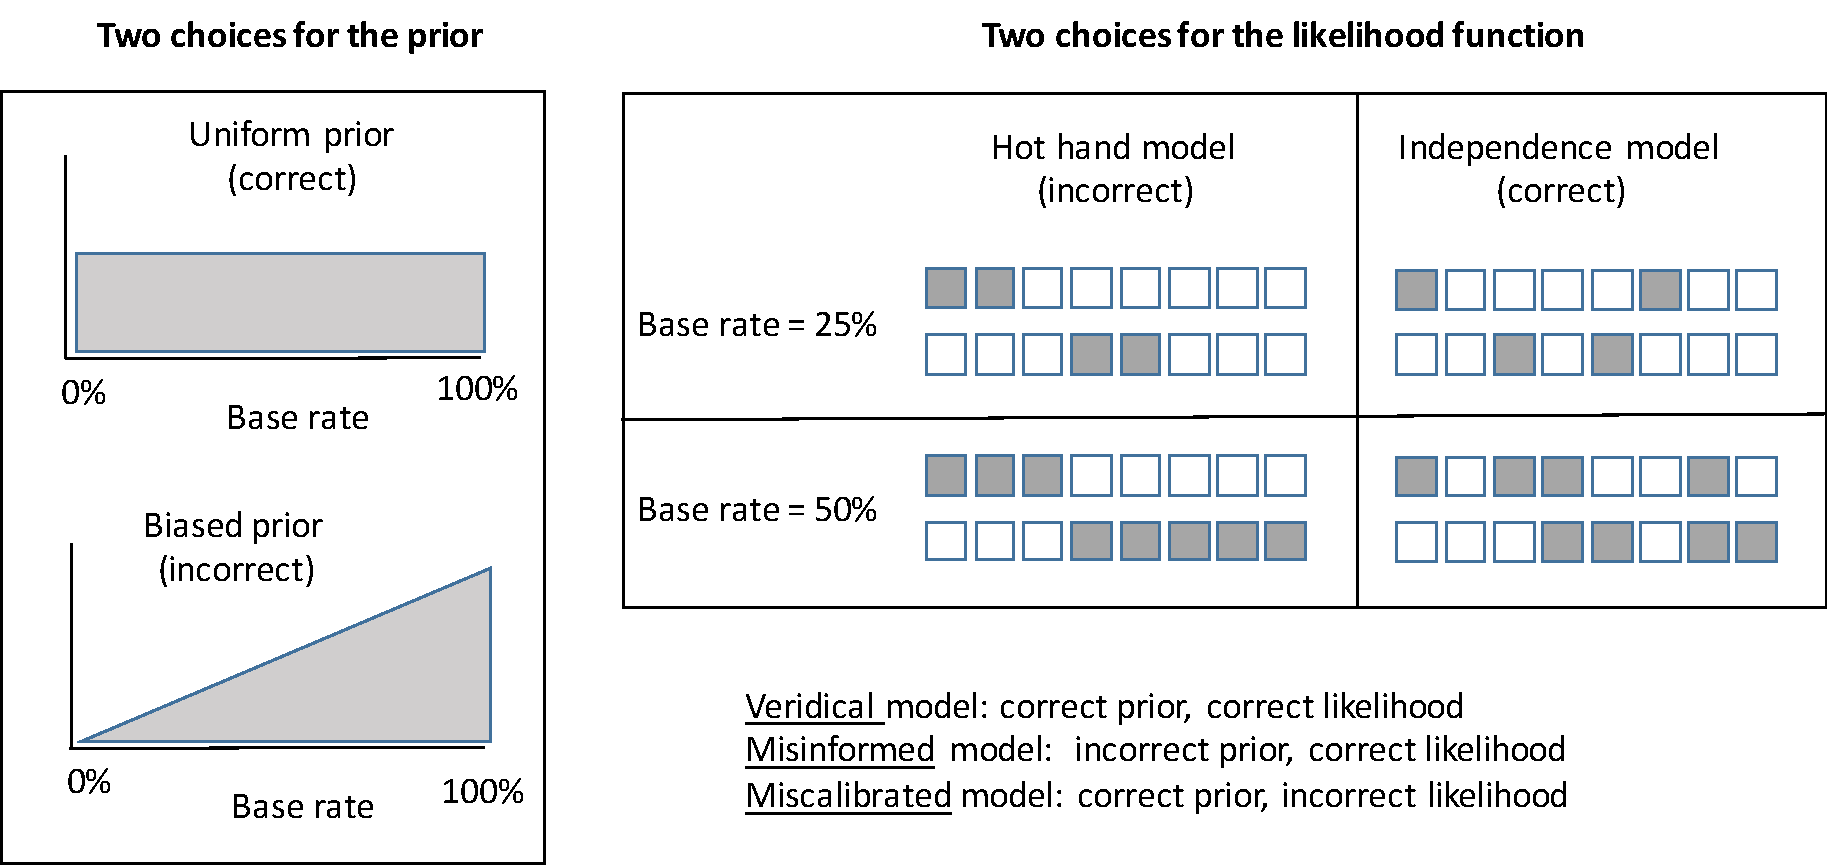
\includegraphics[width=.63\textwidth]{other_figs/threeBayesPic.pdf}}\hspace*{.5cm}
	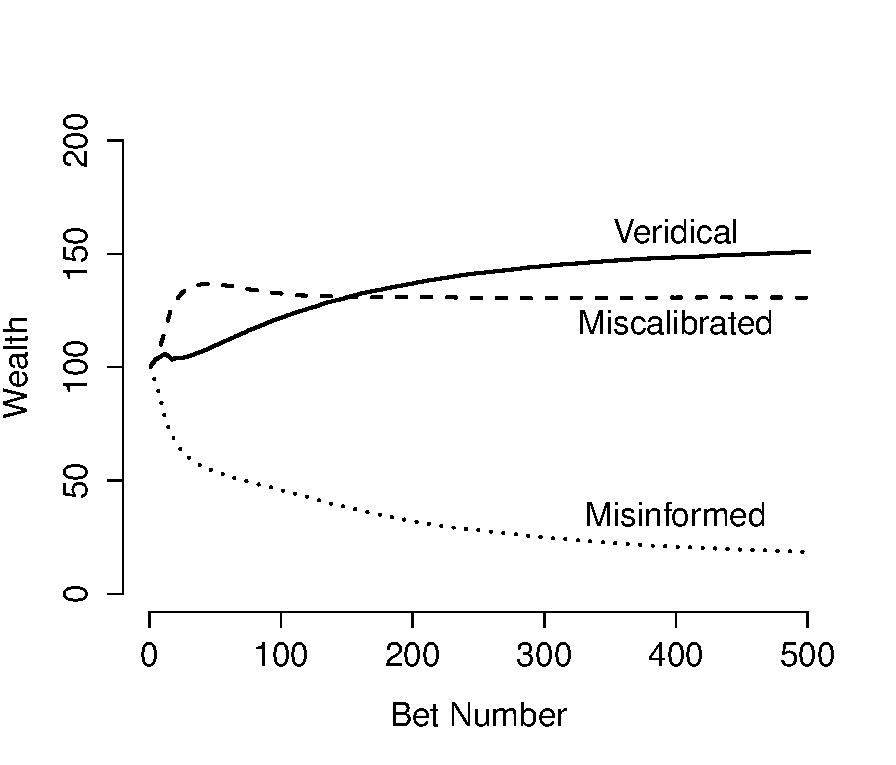
\includegraphics[width=.33\textwidth]{other_figs/threeBayes.pdf}
	\vspace*{6pt}
	\caption{Three Bayesians betting on binary outcomes, where the true success rate $\theta$ is generated randomly from the unit interval. The {\it veridical Bayesian} employs priors and likelihoods that are exactly matched to this task, whereas the {\it misinformed Bayesian} uses the wrong prior and the {\it miscalibrated Bayesian} uses the wrong likelihood. The veridical Bayes outperforms either of the other two models.}
	\label{fig:threeBayes}
	\vspace*{-3mm}
\end{figure}

One of the philosophically appealing features of Dutch book arguments is the fact that this coherence of Bayesian belief revision is an inherent property of Bayes' rule, and not something that is specific to any particular Bayesian model. It is by virtue of this universality that one might argue that all Bayesian models describe a form of rational reasoning, and in one sense it is true. However, it is not at all clear that this kind of rationality is desirable on its own: a Bayesian reasoner whose priors and likelihoods are grossly miscalibrated will find that coherence provides very little protection against losing their money to a better informed agent. In some respects this observation is trite and uninteresting---Teller (1973, p. 224) argues that ``exploitation by dint of such greater knowledge or keener powers of observation shows nothing derogatory about the agent's plan for change of belief.'' In real life, however, few of us would take comfort in such assurances when our incorrect theories about the world lead us to be exploited by others. 

As obvious as this point is, we think it ties naturally to the tension that exists in the cognitive science literature. If a Bayesian reasoner applies priors and likelihoods that are well-matched to the world, they are not merely immune to sure losses via a Dutch book, they also enjoy a practical advantage over their less well-calibrated peers in that they are less likely to be exploited by other agents who happen to have better knowledge. This is highlighted in Figure~\ref{fig:threeBayes} which shows the outcomes of a gambling competition between three Bayesian agents. The competition works as follows: a deck of cards consists of black and white cards with some unknown proportion of black cards (the base rate), and cards are turned over one at a time. Each agent offers what they perceive to be fair bets to the others, and each agent places a \$1 stake on any bet they perceive to be favourable. So if an agent believes that the probability of black to be 0.25 they offer 3:1 odds on black, and place a \$1 bet with any agent offering better than 3:1 odds. The true proportion of black cards is chosen uniformly at random at the beginning of the game, and the cards are perfectly shuffled so that outcomes of successive trials are essentially independent. The {\it veridical} Bayesian agent adopts a prior and likelihood that match this scenario perfectly. The {\it misinformed} Bayesian agent uses the correct likelihood (independent events) but incorrectly believes that the scenario has a bias towards black cards. In contrast the {\it miscalibrated} Bayesian agent has the correct prior beliefs about base rates, but incorrectly believes that the deck of cards has not been properly shuffled and thinks that the cards are likely to show a ``hot hand'' effect in which repetitions are much more common than alternation \cite{gilovich_hot_1985}. This set up is illustrated on the left hand side of Figure~\ref{fig:threeBayes}, and the formal details are outlined in Appendix A. On the right hand of Figure~\ref{fig:threeBayes} we plot the results of simulating a large number of gambling competitions among these three agents. Not surprisingly, although all three are Bayesian models -- and hence ``optimal'' in the sense implied by the diachronic Dutch book argument -- they do not perform equally well in these contests. Early on in the gambling contests, the Bayesian models with the correct prior (veridical and miscalibrated) both tend to win money from the misinformed model because it tends to provide overly generous payouts for a bet on white. As the contest continues, the veridical model starts to win money from the miscalibrated model -- because the miscalibrated model incorrectly believes that a hot hand effect applies it offers and places bad bets reflecting its belief that streaks will tend to continue. While each of these three agents represents an optimal solution to some inference problem, only one of them provides a normative standard for gambling behavior in this specific contest. To our mind, good performance on the actual inference problem at hand seems a very important element of what optimality means in the real world, and it is obvious that the mere fact of being Bayesian is not sufficient to guarantee good performance in any satisfactory sense. To be rational, one must do more than just be Bayesian---one must be the right kind of Bayesian. 
 

The point of this discussion to argue that an {\it optimal} Bayesian model is, in practice and for very good reasons, assumed to be something more than just a model with Bayes' rule in it. At the very least, it refers to a Bayesian model in which the priors and likelihoods are well suited to the experimental task or to a real world problem that the agent needs to solve. It suggests that the builders of such models are obligated to constrain their models by making reference to some external standard that justifies the choice of priors and likelihoods.\footnote{Arguably, a Bayesian who wants to make the strongest possible claim about optimality of  {\it cognition} has an even stronger obligation, namely to show that human behavior matches the predictions of the optimal Bayesian model {\it because} that behavior is optimal. This issue is discussed by \citeA{danks_rational_2008}.} For example, the learner's prior might be veridical in the sense of being the correct prior for the task given to participants (as per the toy example above). Alternatively, a prior might be ecologically justified in the sense that it is well matched to the tasks that people have to solve in their everyday lives. These two need not be identical, and if people apply ecologically justifiable priors in an experimental task for which they are not appropriate, one might argue that the cognition is optimally tuned to the real world problem but not the experimental one. The key point is that if one's Bayesian model is intended to be an optimal Bayesian model, the researcher is not free to choose priors and likelihoods purely on the basis of their own intuitions. Indeed, part of the substantive theoretical claim that Bayesian models are often used to make is about the nature of those priors and likelihoods.


\subsection*{Distinguishing optimality claims from descriptive claims}

The idea that human cognition might be optimal or rational is a powerful thought \cite{cosmides_are_1996}, and there seems little disagreement with the suggestion that there would be considerable scientific value to a demonstration that humans closely mimic the behavior of a genuinely optimal Bayesian model, even if that optimality is defined with respect to constraints on factors like sensory abilities or attentional or memory limitations. Much of the excitement about \cite{Griffiths2006,anderson_reflections_1991,kording_bayesian_2004,chater_probabilistic_2006} and criticism of \cite{bowers_bayesian_2012,Mozer2008} Bayesian theories revolves around the plausibility of this vision, but few would argue that the idea would be boring if true. The dispute arises simply because many cognitive scientists strongly disagree with any claim of human optimality \cite<e.g.,>[p. 393]{bowers_bayesian_2012}, noting that in many tasks human performance appears to be markedly suboptimal \cite<see also>[p. 2353]{marcus_how_2013} when compared to a model that makes the best possible inferences given the structure of the task.

Perhaps suprisingly, some recent defences of the Bayesian framework \cite<e.g.,>{griffiths_how_2012,goodman_relevant_2015} against these criticism have been entirely willing to concede that point. If prominent Bayesian cognitive scientists are prompted to argue that ``the hypothesis that people are optimal is not something that even the most fervent Bayesian believes'' \cite[p. 421]{griffiths_how_2012}, why is there so much confusion in the literature surrounding it? A large part of the problem is that the very structure of Bayesian models---because they require the modeller to stipulate and justify the choice of priors and likeilhoods---encourages an optimal interpretation, even on the part of modellers who did not set out with that goal. Indeed, we would suggest that this characteristic that may have given rise to many of the optimality claims that \citeA{bowers_is_2012} highlighted and found so problematic. In contrast, our {\it descriptive} Bayesian models provide a vision that explicitly, as part of its structure, rejects assumptions or interpretations of optimality. 

If a particular Bayesian model is not intended to constitute a normative claim about what people should do in order to be deemed rational, what purpose does it serve? In our experience, many researchers who develop Bayesian models are quite uninterested in making normative claims. Instead, the goal is merely use the Bayesian framework as a language in which to specify a theory about the learner's mental representations (hypothesis spaces), the beliefs defined using these representations (the priors), and the learning rules that describe how beliefs are revised (the likelihoods). From this perspective Bayesian cognitive models need not correspond to a strong claim about the optimality or rationality of human behavior. Rather, they serve a descriptive goal based on the conditional claim that {\it if} a learner adopted this prior and that likelihood, {\it then} it would be sensible for them to produce that behavior. Viewed in this way it is still critical that Bayesian models be coherent---and Dutch book arguments are still somewhat pertinent---because without such coherence even this conditional claim becomes untenable. However, a learner's prior need not capture the ``correct'' environmental statistics for some problem nor does it need to be veridical for a specific task; it need only capture {\it some} beliefs that the learner might bring to the task \cite<e.g.,>{Hemmer2014,Huszar2010}. Similarly, a likelihood need not describe the ``true'' model in which observations are generated and might not even map onto a particularly sensible one; 
it need only describe how the learner {\it thinks} the observations were generated \cite<e.g.,>{navarro2012}. The hypotheses considered by the learner need not include the {\it best} or most appropriate hypothesis in some objective sense; they need only include some cognitively-plausible set of options a learner might consider. Such a model makes sense on its own terms and serve a useful purpose in illustrating psychological principles, but if the priors or likelihoods are especially mismatched to the task, it is somewhat misleading to refer to such a model as ``rational'' and highly inappropriate to refer to it as ``optimal.'' 

We refer to models constructed in this fashion as {\it descriptive} Bayesian models.\footnote{Sometimes the term `descriptive' is used to capture models that seek to more clearly characterize data (as in, for instance, signal detection or diffusion models) as opposed to models whose aim is to explain the underlying processes or causal relationships. That is not the distinction we are making here. Rather, we use the term to make the distinction between models that seek to describe the priors and likelihoods people actually use, rather than prescribing them {\it a priori} and justifying them as being well-suited to the problem.} Within the descriptive approach, human cognition need not be perfectly matched to the statistics of the environment, people's learning might not make optimal use of the information inherent in the problem, and individual participants might differ quite substantially in their choice of priors and likelihoods. If human behavior matches the predictions made by a model specified in this manner, this is evidence that the model provides a good description of the behavior---which suggests that the model's assumptions may be consistent the assumptions people make in that situation. Critically, good fit of a descriptive model to human behavior does {\it not} imply that the behavior is rational. It is evaluated and interpreted in much the same way as any other probabilistic model of cognition, on a par with models like signal detection theory \cite{macmillan_detection_2004}, sequential sampling theory \cite{ratcliff_comparison_2004}, multinomial processing trees \cite{batchelder_multinomial_1990}, and so on. 

Put another way, the fundamental difference between descriptive Bayesian models and optimal Bayesian models is that within the descriptive Bayesian framework, questions of optimality are simply {\it irrelevant}. This distinction is especially clear when comparing descriptive Bayesian models with models of constrained optimality. The two have sometimes been confused with one another, but they are fundamentally distinct. Models that acknowledge that all optimality occurs within constraints (e.g., investigating whether some behavior is optimal given the existence of certain capacity limitations or filters on the kind of sensory input available) are still optimal models: they still justify the modelling choices by reference to some notion of optimality. That is, the choices of priors, likelihoods, hypotheses, or characteristics are justified by arguing that they are well-matched to the task or in some other way ecologically valid, given the constraints the organism is operating within. A descriptive approach, by contrast, simply doesn't {\it care} whether the choices are justified. The central question of interest is discovering what choices best account for human performance. 

This raises the question: if the descriptive approach liberates Bayesian models from the requirement that they be ``rational'' or ``optimal'', why should a researcher adopt such an approach? What are the virtues of Bayesian models if they no longer represent optimal inference or produce rational behavior? It might appear that we are discarding the core virtue of Bayesian models. Yet this is far from the case. Much of the appeal of Bayes' rule lies in the fact that it represents a method for writing down models in a transparent way. To build a Bayesian model, the researcher is forced to specify what form the mental representation might take (the hypothesis space), what biases the learner brings to the problem (the prior), and the rules by which the learner can be influenced by data (the likelihood). Because the researcher cannot write down a Bayesian model without making these things clear, the assumptions of the theory are always out in the open. Such a model tries to explain human behavior in much the same way any other model does: If the learner possesses {\it these} beliefs and reasons in {\it this} way, it would be reasonable to expect them to produce {\it that} behavior. 

How, then, are descriptive Bayesian models different from modelling more generally? In one sense they are just one of many options in our toolbox; which approach should be used depends on the research question. But the particular research questions a descriptive approach are well-suited for are exactly the kinds of questions that often arise in cognitive science. What is the nature of the hypotheses people are evaluating when they learn? How exactly do people update their beliefs in response to the data they see, and what assumptions do they make about how that data was generated? What priors do people bring to a learning situation? These questions are more naturally answered within a descriptive framework than an optimal one, and the explicitness of the Bayesian machinery means that for those kinds of questions it can offers advantages of explicitness and precision over other modelling frameworks as well. 



\subsection*{A formal statement of the descriptive Bayesian approach}

Relaxing the requirement that Bayesian models describe optimal cognition opens up the possibilities for investigation considerably. In an optimal Bayesian model, the learner's inferences are described via the application of Bayes' rule:
\be
P(h|x) = \frac{P(x|h)P(h|\mathcal{H})}{\sum_{h^\prime \in \mathcal{H}} P(x|h^\prime)P(h^\prime|\mathcal{H})}
\label{eq:obmc}
\ee
where $x$ represents the data available to the learner, $h$ is a hypothesis about the origins of the data, and $\mathcal{H}$ represents the set of hypotheses available to the learner. In order to satisfy some version of the optimality claim, the priors and likelihoods need to be constrained in an a priori fashion.

The descriptive view rejects the idea that priors and likelihoods should be constrained by anything beyond the researcher's theory of the task. The learner's prior should not be viewed as fixed by the structure of the environment, nor should it necessarily correspond to a sensible expectation about the world. Similarly, the likelihoods that govern people's learning need not correspond to any realistic model of how observations are generated. As such, the behavior produced by the model need not be rational or even particularly sensible. Formally, if there are multiple possible choices of prior (parameterized by $\phi$) and likelihoods (parameterized by $\lambda$), then the learner's inferences are conditioned on these parameters:
\be
P(h|x,\lambda,\phi) = \frac{ P(x|h,\lambda) P(h | \phi, \mathcal{H}) }{\sum_{h^\prime \in \mathcal{H}} P(x|h^\prime, \lambda) P(h^\prime|\phi, \mathcal{H})}
\label{eq:ddbmc}
\ee
In one sense the difference between these two expressions is purely cosmetic: Equation~\ref{eq:obmc} suppresses the dependence on the parameters $\phi$ and $\lambda$, whereas Equation~\ref{eq:ddbmc} makes the dependence explicit. However, this distinction is central to the manner in which a descriptive Bayesian model differs from a traditional rational analysis. If the purpose of a Bayesian model is to make claims about optimality, the parameters $\phi$ and $\lambda$ are nuisance variables that (ideally) should be fixed by reference to some external standard. However, if the purpose of a Bayesian model is to help us develop good descriptions of human cognition, the core goal is now to {\it learn} what priors and likelihoods people rely on. Inferring the priors $\phi$ and likelihoods $\lambda$ from the empirical data is now the aim.\footnote{It should be noted that this is a slight oversimplification. For instance, in some situations (e.g., our case study 3) the goal is to infer the {\it hypothesis space} $\mathcal{H}$. The notation could be expanded to express this but for expositional simplicity we suppress this for now.} 

W can illustrate the difference between a descriptive and optimal model with a simple category learning example. If the researcher is operating within an optimal Bayesian framework, when they specify their model they should consider what kinds of category-learning priors would be optimal: for instance, they might incorporate a prior that favors more coherent categories \cite{rosch78} on the grounds that such a category system is sensible \cite{navarro_hypothesis_2011}. They should also consider what kinds of likelihood models an optimal learner should entertain: perhaps one that assumes strong sampling and follows the size principle on the grounds that it is statistically appropriate if one assumes that data is drawn directly from the category itself \cite{Tenenbaum2001}. The key point is that an optimal Bayesian modeller needs to not only make choices about the prior and likelihood, but they should be able to justify those choices as optimal for some reason. By contrast, a descriptive Bayesian modeler need not do this. Instead, they perform inference {\it over} the priors and likelihoods\footnote{As we describe in more detail below, it is of course impossible to perform inference without setting some hyper-prior on the priors and likelihoods themselves. Yet these hyper-priors can be loose enough to permit a large range of variation in the actual priors and likelihoods entertained by the model. As such, they themselves need to be justified on optimality grounds, and they allow the researcher to truly do inference about which parameters best describe human performance} of each participant and discover which ones best account for their performance. Perhaps some people use strong sampling, while others do not; perhaps everybody, or nobody, or a few people do not have particularly strong {\it a priori} beliefs about the coherence of categories. The descriptive approach allows researchers to discover this. 

The descriptive approach to Bayesian cognitive modeling allows the researcher a lot of freedom in how the model can be built and parameterized, so it becomes critical to consider how the model parameters should be estimated and how rival models should be compared. Fortunately, these are well-studied problems and many principled solutions exist for model selection   \cite<see e.g.,>{browne_cross-validation_2000, pitt_global_2006, pitt_toward_2002, myung_importance_2000, myung_model_2006, wasserman2000bayesian, Shiffrin2016, ShiffrinInPress, ChandramouliInPress}, and perhaps the most elegant approach to parameter estimation is Bayesian data analysis \cite<e.g.,>{lee_bayesian_2014, kruschke_doing_2010, gelman_bayesian_2014}, in which the {\it researcher} also acts as a Bayesian reasoner. Before running any experiment, the researcher themselves has some priors $P(\lambda,\phi)$ that captures their beliefs about which priors and which likelihoods are plausible. After running the experiment she obtains a collection of responses $r$ from the participant, from which she infers a posterior distribution $P(\lambda,\phi|r)$. This distribution captures everything the researcher has learned about the participant using her model and the data from her experiment. The inference by the researcher can also be described using Bayes' rule,
\be
P(\lambda,\phi | r) = \frac{P(r|x,\lambda,\phi)P(\lambda,\phi)}{\int P( r| x,\lambda^\prime,\phi^\prime) P(\lambda^\prime,\phi^\prime) \ d(\phi^\prime, \lambda^\prime)}
\ee
In this expression, we use the notation $P(r | x,\lambda,\phi)$ to indicate that the participant responses $r$ depend on both the parameters $(\lambda,\phi)$, and on the information $x$ that the experiment presents to the participant. In order to do so, the researcher needs to specify two things. Firstly, as noted above, she needs to specify the prior distribution over model parameters, $P(\lambda,\phi)$. Secondly, she needs to specify a data analysis model that links the learner's posterior distribution over hypotheses $P(h|x,\lambda,\phi)$ to the researcher's likelihood function for the data, $P(r | x,\lambda,\phi)$. Specifying the data analysis model requires the researcher to make substantive choices. For instance, one might assume that people generate their response by sampling from the posterior \cite<e.g.>{vul_one_2014}, but other possibilities exist. Several simple possibilities are listed by \citeA{marcus_how_2013}, but there is no reason why a complex theory of the response generation process could not be supplied \cite<see e.g., the Appendix in>{navarro2012}. The important point is that if the researcher does specify a clear measurement model that links the learner's posterior $P(h|x)$ to the observed responses $r$, then all of the statistical machinery of Bayesian data analysis and other approaches to model selection now become available. 


\subsection*{Summary}

The descriptive approach to Bayesian cognitive modeling has many fundamental differences from a view in which Bayesian models are treated as optimal, normative standards for human cognition. Firstly, the descriptive approach treats the cognitive model as a {\it tool} to make inferences about participants. When building a model, the researcher is not obligated to have a theory that precisely states what priors and likelihoods a learner should use. Instead, they can propose a broad family of possible Bayesian models and use the experimental data to infer which of those models best matches human behavior. Secondly, it provides a natural mechanism for expressing individual differences, as it allows each participant to have different priors $\phi$ and likelihoods $\lambda$ without obligating the researcher to suppose that each person's idiosyncratic prior and likelihood is fully justified given their idiosyncratic experiences. Thirdly, because the descriptive framework emphasizes the importance of treating the Bayesian cognitive model as a genuine statistical model for the data (i.e., ideally, it assigns probabilities to people's responses at a trial to trial level), we can use a number of model selection approaches, including methods from Bayesian statistics, to compare between models of different sorts (even if some of those models are non-Bayesian). 

The primary goal in this paper is to highlight the importance of making a clear {\it distinction} between an optimal Bayesian model and a descriptive one, and the rest of the paper is devoted to illustrating why this distinction matters. To that end we present three case studies. Our first case study presents an example in which an optimal Bayesian model fails to account for human behavior, whereas a descriptive Bayesian model performs better---by dropping the presumption of optimality and allowing for individual differences---and yields novel insights into how people solve a simple inductive problem. The second case study presents an example in which the comparison between an optimal Bayesian model, a descriptive Bayesian model, and a non-Bayesian model explores how close people actually are to optimal in some cases. This case study illustrates that even when people's behavior is {\it actually} close to optimal, the descriptive framework is still useful. Not only does it provide a framework for making the  comparison, but it also constitutes {\it better} evidence for optimality than an optimal model alone would: the priors and likelihoods that correspond to the normative solution are rigorously shown to provide the best account of the data, rather than being simply stipulated by the modeller. Finally, our third case study highlights the fact that descriptive Bayesian models can still be useful in situations where exploring whether or not people are optimal is irrelevant to the research question.


These examples are intended to be illustrative, not exhaustive. We aim to highlight the potential power of the descriptive approach, not to catalog all possible uses of the framework. Although there are a number of important technical details to consider when applying Bayesian data analysis to a Bayesian cognitive model, we have aimed to keep these technical details to a minimum in the main paper, but more fully elaborated in the Appendices. Finally, we should note that although our examples are chosen to illustrate why it can be useful to build descriptive Bayesian models, we believe that there is a place for both kinds of Bayesian models in the literature. For instance, optimal Bayesian models are quite appropriate in cases where the modeller has independent substantive justification for the choice of likelihoods and priors; in such a situation, the extra machinery of the descriptive approach may be unnecessary.



